\documentclass{beamer}
%\usetheme{CambridgeUS}
\usetheme{Warsaw}
\usepackage[utf8]{inputenc}
\usepackage{polski}
\usepackage[polish]{babel}
\usepackage[OT4]{fontenc}
\usepackage{graphicx}
\usepackage{listings}

\newtheorem{hypothesis}{Hipoteza}

\author{Konrad Gądek}
\institute[AGH]{Akademia Górniczo-Hutnicza}
\date{12.~stycznia 2011.}
\title{Obliczenia numeryczne w~języku Java}
\begin{document}

\section*{Wprowadzenie}
\begin{frame}
	\titlepage
	\tableofcontents
\end{frame}

\section{Liczby zmiennoprzecinkowe}

\begin{frame}{IEEE 754 vs. Java}
	\begin{enumerate}
		\item[\#0.] Obsługa \texttt{float} ale brak \texttt{double} (procesory sygnałowe).
		\item[\#1.] 4--bajtowy \texttt{float} i~8--bajtowy \texttt{double} (RISC).
		\item[\#2.] To, co w~\alert{\#1} oraz operacja łącznego mnożenia--dodawania (Power--PC, MIPS R\dywiz 10000).
		\item[\#3.] To, co w~\alert{\#1} oraz +10--bajtowa \texttt{long double} (Intel x86, Motorola 680x0).
	\end{enumerate}
	\begin{alertblock}{Java}
		JVM jest elementem \#$\frac{1}{2}$~--- nie obsługuje ani ,,\emph{Exception Flags}'' ani ,,\emph{Directed
		Roundings}''.
	\end{alertblock}
\end{frame}

\begin{frame}{Traps, Exception Flags}
	\begin{block}{Nazewnictwo IEEE 754.}
		\begin{enumerate}
			\item Trap
			\item Exception Flags \texttt{(Overflow, Underflow, Invalid Operation, Division by zero,
				Inexact Result)}.
		\end{enumerate}
	\end{block}
	\begin{alertblock}{Nazewnictwo w~Javie.}
		\begin{enumerate}
			\item Exceptions
			\item \alert{brak odpowiednika}
		\end{enumerate}
	\end{alertblock}
\end{frame}

\begin{frame}{Traps, Exception Flags}
	\begin{itemize}
		\item Z~poziomu Javy nie ma dostępu do Exeption Flags.
		\item Flagi zostały wprowadzone do IEEE 754. dlatego, że okazały się w~praktyce niezbędne.
		\item Eksperci są często w~stanie znaleźć (\texttt{skompilowane}) algorytmy niewymagające tych flag.
	\end{itemize}
	\begin{block}{Jakie może mieć skutki brak poprawnej obłsugi flag?}
		Takie miało w~języku \texttt{Ada} \scriptsize{(Integer Overflow przy konwersji z~\texttt{float})}:\\
		\centerline{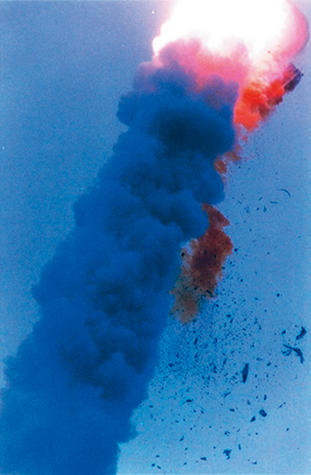
\includegraphics[scale=0.18]{ariane.jpg}}
	\end{block}
\end{frame}

\begin{frame}{strictfp a~powtarzalność obliczeń}
	\begin{block}{By wszystkim żyło się lepiej\ldots}
		Wszystkie wyniki pośrednie są obcinane do 64--bitów.
	\end{block} \ \\
	Obecnie:
	\begin{itemize}
		\item Od JVM 1.1 ~--- domyślnie wykorzystywanie dokładniejszych wyników pośrednich
		\item Stare zachowanie można wymusić flagą \emph{strictfp}.
	\end{itemize}
\end{frame}

\section{Inne aspekty}

\begin{frame}{Skalowalność, wydajność, biblioteki}
	\begin{itemize}
		\item Biblioteki - są, ale najwięcej bibliotek dla Fortrana / C / C++.
		\item Skalowalność - przenośność i RMI (\texttt{Remote Method Invocation}) ale RMI zbyt wolny.
		\item Wydajność - nie jest źle, ,,\emph{ale}''\ldots
	\end{itemize}
\end{frame}

\section{Podsumowanie}

\begin{frame}{Podsumowanie}
	\begin{itemize}
		\item Brak zgodności ze standardem IEEE 754.
		\item Mniejsza ilość bibliotek numerycznych niż w~wypadku Fortrana / C / C++\ldots ?
		\item Problemy ze skalowalnością\ldots ?
		\item Gorsza wydajność\ldots ?
		\item Brak \texttt{long double}\ldots
		\item \ldots a~co z~technologią CUDA?
	\end{itemize}

	\begin{block}{Czy Java jest bezużyteczna?}
		Juan Villacis pokazał, że Java nadaje się jako pośrednik (tzw. ,,\texttt{glueware}''), do pisania
		programów ,,wokół'' programów właściwych.
	\end{block}
\end{frame}

\begin{frame}{Bibliografia}
	\begin{itemize}
		\item{Prof. Kahan and Joseph D.~Darcy. ``\emph{How Java's floating point hurts Everyone Everywhere}''.
			Workshop on Java for High--Performance Network Computing, ACM 1998.}
		\item{Juan Villacis. ``\emph{A Note on the Use of Java in Scientific Computing}''.
			ACM SIGAPP Applied Computing Review, volume 7 Issue 1, 1999.}
		\item{Kanał \#java na irc.freenode.net}
	\end{itemize}
	\ \\
	\texttt{http://student.agh.edu.pl/\textasciitilde gadek/3\_mownit/prezentacja.pdf}
\end{frame}

\end{document}

